 \documentclass[12pt]{article}
 \usepackage[
    left=1.25in,
    right=1.25in,
    top=1.5in,
    bottom=1.5in]{geometry}

\usepackage[english]{babel}				% orthography
\usepackage[T1]{fontenc}
\usepackage{lmodern}				% font family
\usepackage{microtype}				% for micro typography (for a better typeface)
\usepackage{blindtext}

\usepackage{longtable} 		
\usepackage{multicol}				
\usepackage{multirow}
\usepackage{booktabs}
\usepackage{tabularx}
\usepackage{xcolor}
\usepackage{varioref}
\usepackage[active]{srcltx}
\usepackage{listings}				% algorithm
\usepackage{mdwlist}				% lists

\usepackage{setspace} 				% setting of the lines (rows)
\newtheorem{mydef}{Merksatz}  		% if examples or mnemotechnic verses are used with continuous numeration 
\newtheorem{bsp}{Beispiel}

\usepackage{calc}
\usepackage{tablefootnote}			% footnotes in tables
\hyphenation{voll-st\"andigen}		% for defining word devisions globally

\usepackage[utf8]{inputenc}
\usepackage{amsmath}
\usepackage{graphicx}
\graphicspath{{./Graphics/}}          % path to the pictures

\usepackage[hidelinks]{hyperref}
\hypersetup{
    colorlinks=true,
    linkcolor=blue,
    filecolor=magenta,      
    urlcolor=cyan,
    citecolor=blue,
    pdfborderstyle={/S/U/W 0}
}

\usepackage[round]{natbib}
\bibliographystyle{plainnat} % Use any other style like abbrvnat if desired

\begin{document}

% Title page shall not include header or foooter lines
\thispagestyle{empty}

% All elements shall be centered
\begin{center}

    \vspace*{-8mm}

    {\LARGE INSTITUTE OF FINANCE AND STATISTICS\\[1mm]}
    \large University of Bonn\\

    \vspace*{1cm}

    
\includegraphics[width=0.4\textwidth]{./Graphics/UNI_Bonn_Logo_Standard_RZ.eps}

    \vspace*{1cm}

    % Kind of Thesis => (Bachelor Thesis ,Diploma Thesis, Master Thesis, Seminar Thesis)
    {\Large \textbf{Seminar Paper in Academic Practice}}\\

    \vspace{1cm}

    % Title of the Thesis
    {\Large \textbf{Regression Trees}}\\
    \vspace{1.5cm}

    % Names of Authors
    {\LARGE Timothy Currie}\\[15mm]

    % Superverisor, contact data and submission date
    \parbox{120mm} {
        \begin{large}
            \begin{tabbing}
                Supervisor: \hspace{1.8cm} \= Dr. Elias Wolf\\[1.5mm]
                Semester:\> Summer Term 2024\\[1.5mm]
                Author:\>Timothy Jakob Currie\\[1.5mm] % alphabetic order (Surname)
                Matriculation-Nrs.:\> 50074426\\[1.5mm]
                %Address:\> Street Nr, Postal Code City\\[1.5mm]
                Email:\> s69tcurr@uni-bonn.de\\[1.5mm]
                Subject:\>Bachelor Economics\\[1.5mm]
                Submission:\> 25. August 2024\\[1.5mm]
            \end{tabbing}
        \end{large}
    }

\end{center}
\clearpage{\pagestyle{empty}\cleardoublepage}


\pagenumbering{arabic}% Arabic and reset to 1)

\begin{abstract}
Test13. Modern economic research heavily relies on linear regression.
However, to conduct effective economic research, it is crucial to understand both the strengths and weaknesses of linear regression, as well as where it outperforms or is outperformed by other methods. This paper explores Regression Trees as an alternative to linear regression . In it I will explain the theory behind regression trees and compare them to linear regression using a series of simple simulations, focusing on interaction effects and pruning. The paper also highlights extensions to regression trees that enhance their performance. Subsequently, both methods are applied to a dataset of student performance, emphasizing the strengths and weaknesses of linear regression and tree-based methods.
\end{abstract}

\newpage

\tableofcontents

\newpage


\section{Introduction}
While linear regression is arguably the most frequently used method by empirical economists and can be valuable in many situations, it is essential to examine its limitations and areas where alternative methods excel. Regression trees have emerged as a powerful machine learning technique for predictive modeling, with numerous extensions greatly improving their utility. Regression trees offer an alternative approach that can be beneficial in various scenarios. This paper will discuss their advantages over traditional linear regression methods, cover the fundamentals of regression trees, compare them with linear regression, address the issue of overfitting, and introduce advanced ensemble methods such as Bayesian Additive Regression Trees (BART).



In this paper I will first give a brief exposition on Regression Trees, their theory, extensions and applications and contrast them with linear regression. I will perform easily interpretable simulations comparing Regression Trees and Linear Regression. Show how Regression Trees can be used on a Dataset of information about students and their test performance.

Given the widespread use of linear regression, it is particularly important to identify where it performs well and where it falls short, as well as where other methods can improve upon it. Due to their interpretability, trees may also serve well in educational roles.

Linear regression performs poorly on many types of data, particularly those with non-linear relationships and interaction effects. Regression Trees can be useful in many situations where linear regression falls short.

Since \citep{breiman1984} presented the CART algorithm there has been a lot of work on various Tree based methods.

\citep{hastie2021} serves as an excelent modern introduction to Regression trees, while while \citep{tan2019} give a deeper dive on BART a powerful ensemble method. 
Random forests, a very popular Tree based ML method are explained very well in\citep{biau2016}.



I found how simulations are good at showcasing model in an ideal setting. The simulations show how regression trees outperform linear regression on datasets with non liner relationships. etc. And how pruning can help find the optimal tradeoff between overfitting and not capturing enought of the signal. While applying the methods to the real world data can showcase how trees capture  interaction effects and how pruning works I discovered. Also the complications of worknig with real world data, as opposed to simulations.

  
In section 2 I will give a brief overview of the theory of regression trees, and where and where not we might expect them to perform will. And will also explain the bias variance trade-off and explain how pruning helps and ensemble methods that are extensions to trees.

In section 3 I will run a number of simulations comparing RRTT and LLRR and showcasing different aspects of RRTT under ideal conditions.

In section 4 I will apply these methods to a dataset of student test performance. Paying special attention to overfitting pruning and test vs validation vs training set. Also showing some of the shortcomings of RRTT and using BART.

Section 5 is the conclusion and will sum up what I have found and further interesting areas where research could be done.

This dataset used in this paper is publicly available at \href{https://www.kaggle.com/datasets/uciml/student-alcohol-consumption}{Kaggle: Student Alcohol Consumption Dataset}. All code used for the simulations and data analysis is avialible at \href{https://github.com/Tim2othy/wissenschaftliches-arbeiten}{my GitHub}.



\section{Regression Trees}

Regression Trees are a type of supervised machine learning algorithm that recursively splits the predictor space into smaller rectangular subregions. This process approximates an unknown function $f$ by minimizing a measure of loss at each split. Unlike linear regression, Regression Trees don't make assumptions about linearity or non-interaction between different dimensions, making them particularly useful for complex, non-linear relationships in data.

The core mechanism of Regression Trees involves splitting the predictor space into regions that minimize the residual sum of squares, given by:

\begin{equation}
    \sum_{j=1}^{J} \sum_{i \in R_j} ( y_i- \hat{ y}_{R_j} )^2
\end{equation}



In each region, $\hat{y}$ simply takes on the mean of all observations in that region.
Each branching of the tree divides the predictor space into two regions, for numerical variables typically of the form $\{x \le c\}$ or $\{x > c\}$. In each resulting region, the predicted value $\hat{y}$ is simply the mean of all observations within that region.

The algorithm employs a greedy approach called Recursive binary splitting to find the optimal split at each stage to minimize prediction error. This process continues until a specified threshold is reached, such as a minimum number of observations in each leaf node or a maximum tree depth.

\begin{figure}\centering
    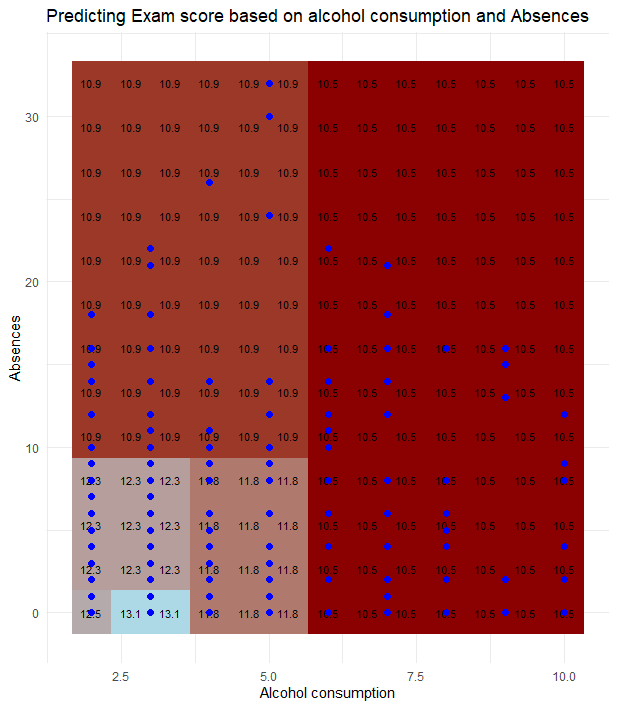
\includegraphics[scale=0.40]{waste_of_time.png}
    \caption{Visualization of Regression Tree's predictions}
\end{figure}


Regression Trees offer several advantages over traditional linear regression methods. They can capture non-linear relationships between predictors and the response variable without requiring explicit specification of these relationships. Furthermore, they naturally account for interaction effects. For instance, if being blonde typically increases pay, but only for women, a Regression Tree will often automatically split along gender and then, for women only, along hair colour. This ability to model complex interactions without manual specification is a significant strength of the method.



One other major benifit of Trees over Linear Regression is thet they capture interaction effects naturally. If for example being blong typically increases pay, but only for women, a Regression Tree will ofnet naturally split along gender and then, for women only, along haircolor. Whereas in a linear Regression the researcher would have to manually include terms for all interaction effects they want to study.
However, Regression Trees are not without challenges. One of the primary issues is their tendency to overfit the data, especially when allowed to grow deep. Unlike linear regression, where overfitting primarily occurs with high-dimensional data, regression trees can overfit even with low-dimensional data. This is because they have the flexibility to create very specific rules that may capture noise in the training data rather than true underlying patterns.


\begin{figure}
    \centering
    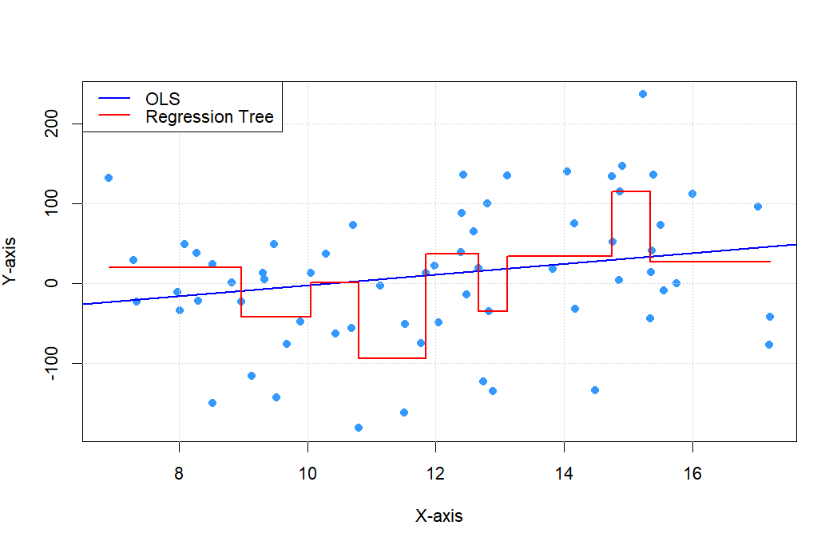
\includegraphics[scale=0.50]{image.png}
    \caption{Regression Tree overfitting}
\end{figure}



\subsection{Pruning}

To address the issue of overfitting and improve overall performance, researchers have developed methods to "prune" regression trees. One of the most effective techniques is cost complexity pruning. This process involves several steps:

First, a large tree is grown that is likely to overfit the training data. Then, a complexity parameter $\alpha$ is introduced to penalize the tree's size. The pruning process is guided by the following formula:

\begin{equation}
    \sum_{m=1}^{|T|} \sum_{i: x_i \in R_m} (y_i - \hat{y}_{R_j})^2 + \alpha|T|
\end{equation}



Where $|T|$ is the number of terminal nodes in the tree. For each value of $\alpha$, the algorithm finds the subtree that minimizes this cost function. The optimal $\alpha$ is then selected using cross-validation, which helps achieve a good trade-off between bias and variance. The larger the cost complexity parameter $\alpha$, the better each split has to be to justify its existence. Recursivly the least important split is removed. As one prunes a large tree by increasing $\alpha$, the tree is naturally pruned in a predictable and well-behaved fashion, allowing one to select the preferred tree.




Instead of evaluating a model on the data we trained it on, we evaluate it on a separate set. In the `rpart` library, cross-validation is performed, and the error for all different trees is produced right away, allowing one to select the tree that performs best on the cross-validation error. This lets one achieve a good trade-off between bias and variance. A large $\alpha$ results in very small trees, while a small $\alpha$ results in larger trees.


\subsection{Ensemble Methods}
While pruning can significantly improve the performance of individual regression trees, they often still underperform compared to other advanced machine learning methods. This limitation led to the development of ensemble methods, which combine many regression trees to create more robust and accurate predictions. As Condorcet's jury theorem shows, if predictors are uncorellated and each predictor's answer is better than pure chance adding more predictors will increase the quality of the average of all answers \citep{condorcet1785}.

Ensemble methods improve results by leveraging the "wisdom of crowds" effect. If each tree has, for example, a 70\% chance of being correct, and the errors are uncorrelated, combining many trees will tend to improve overall accuracy. The two main approaches to creating ensembles are:

1. Growing many independent trees and averaging them. Random Forests are a very popular ML method that does this.
2. Growing trees on the residuals of the current tree model, as in boosting methods or Bayesian Additive Regression Trees (BART).

Random Forests create an ensemble by growing many decorrelated trees. Each tree is trained on a random subset of the training data and is only allowed to consider a random subset of features at each split. The final prediction is then formed by averaging the predictions of all trees (typically around 500). This approach reduces overfitting while maintaining the ability to capture complex patterns in the data \citep{biau2016}.

I will go into slightly more detail for the BART method, as that is the extension I used on the dataset. BART model the data as a sum of many Trees plus noise:

\begin{equation}
    Y_i = \sum_{j=1}^{m} g(X_i; T_j, M_j) + \epsilon_i
\end{equation}


Where $m$ is the number of trees, typically around 200. And $g(X_i; T_j, M_j)$ represents the contribution of the $j$-th tree. $T_j$ and $M_j$ represent the tree's structure and predictions respectively. And $\epsilon_i$ is the noise term.

The BART algorithm proceeds by first generating e.g., 200 trees, without any splits. For each Tree $j$, it calculates the residual error $R_{-j}$ by taking in all the current trees except $j$:


\begin{equation}
R_{-j} = Y - \sum_{t\not=j} g(X,T_j,M_j).
\end{equation}



Then it proposes a change to that tree's structure, such as pruning a node, growing a node, or changing some splitting rule. It then accepts or rejects this modification based on its posterior probability. Which variable will be used is randomly selected to serve as the splitting variable, similar to random forests. If one averaged many trees but did not ensure they are uncorrelated, most of them might make the exact same split, thereby eliminating their wisdom of crowds. This process is repeated for all $m$ trees. That constitutes one iteration of the algorithm. Typically, BART uses 1000 burn-in iterations followed by 1000 sampling iterations. An estimate for f(x) can be obtained not by simply taking the final sum of trees the last iteration produced, but by taking the average over all sample iterations, discarding the burn-in iterations.

A more complete exposition can be found in Chipman et al. (2010). of the BART method and how it's Bayesian.

The algorithm then uses Markov Chain Monte Carlo (MCMC) sampling to draw from the posterior distribution of the model parameters.

BART uses a Bayesian approach, specifying priors on the tree structures, terminal node parameters, and error variance. Nodes at depth $d$ are nonterminal with probability $\alpha(1 + d)^{-\beta}$. This prior on shallow trees makes them be weak learners, more suited to being averaged. Each tree explains a small different part of $f$. It also has other priors that inform how it assigns estimates to the terminal nodes, but that is beyond the scope of this paper.

Default values for these hyperparameters of $\alpha = 0.95$ and $\beta = 2$ are recommended by \citep{chipman2010}. Default values generally provide good performance, but optimal tuning can be achieved via cross-validation. !!!!

Ensemble methods like Random Forests and BART have shown remarkable success in various applications, often outperforming individual regression trees and even many other machine learning techniques. They offer a powerful toolset for modeling complex relationships in data, providing both predictive accuracy and, in the case of BART, measures of uncertainty.

In conclusion, while individual regression trees offer interpretability and the ability to capture non-linear relationships, their tendency to overfit can limit their effectiveness. Pruning techniques help mitigate this issue, but ensemble methods take the concept further, leveraging the strengths of multiple trees to create highly accurate and robust models. The choice between these methods depends on the specific problem at hand, the importance of interpretability, and the need for uncertainty quantification in predictions.





\section{Simulations}

Simulations can serve as a testing ground for statistical methods, allowing for easier repeatability and eliminating many of the complications that arise when using datasets. Simulations are especially useful in comparing two different methods. Here, I will compare Linear regression and regression trees on linear and non-linear data.

\subsection{Linear Data}


This first simulation shows where linear regression excels and trees aren't especially useful. The data follows a simple linear relationship, exactly as the normal least squares regression assumes it does. The data was generated as: $Y = \beta_0 + \beta_1X + \epsilon$, with epsilon normally distributed. I ran the simulations 400 times with regression trees, having 4 terminal nodes. And compared the Mean Squared Error (MSE) for both methods. The attached figure quite clearly shows how linear regression is more suited to this data.


\begin{figure}
    \centering
    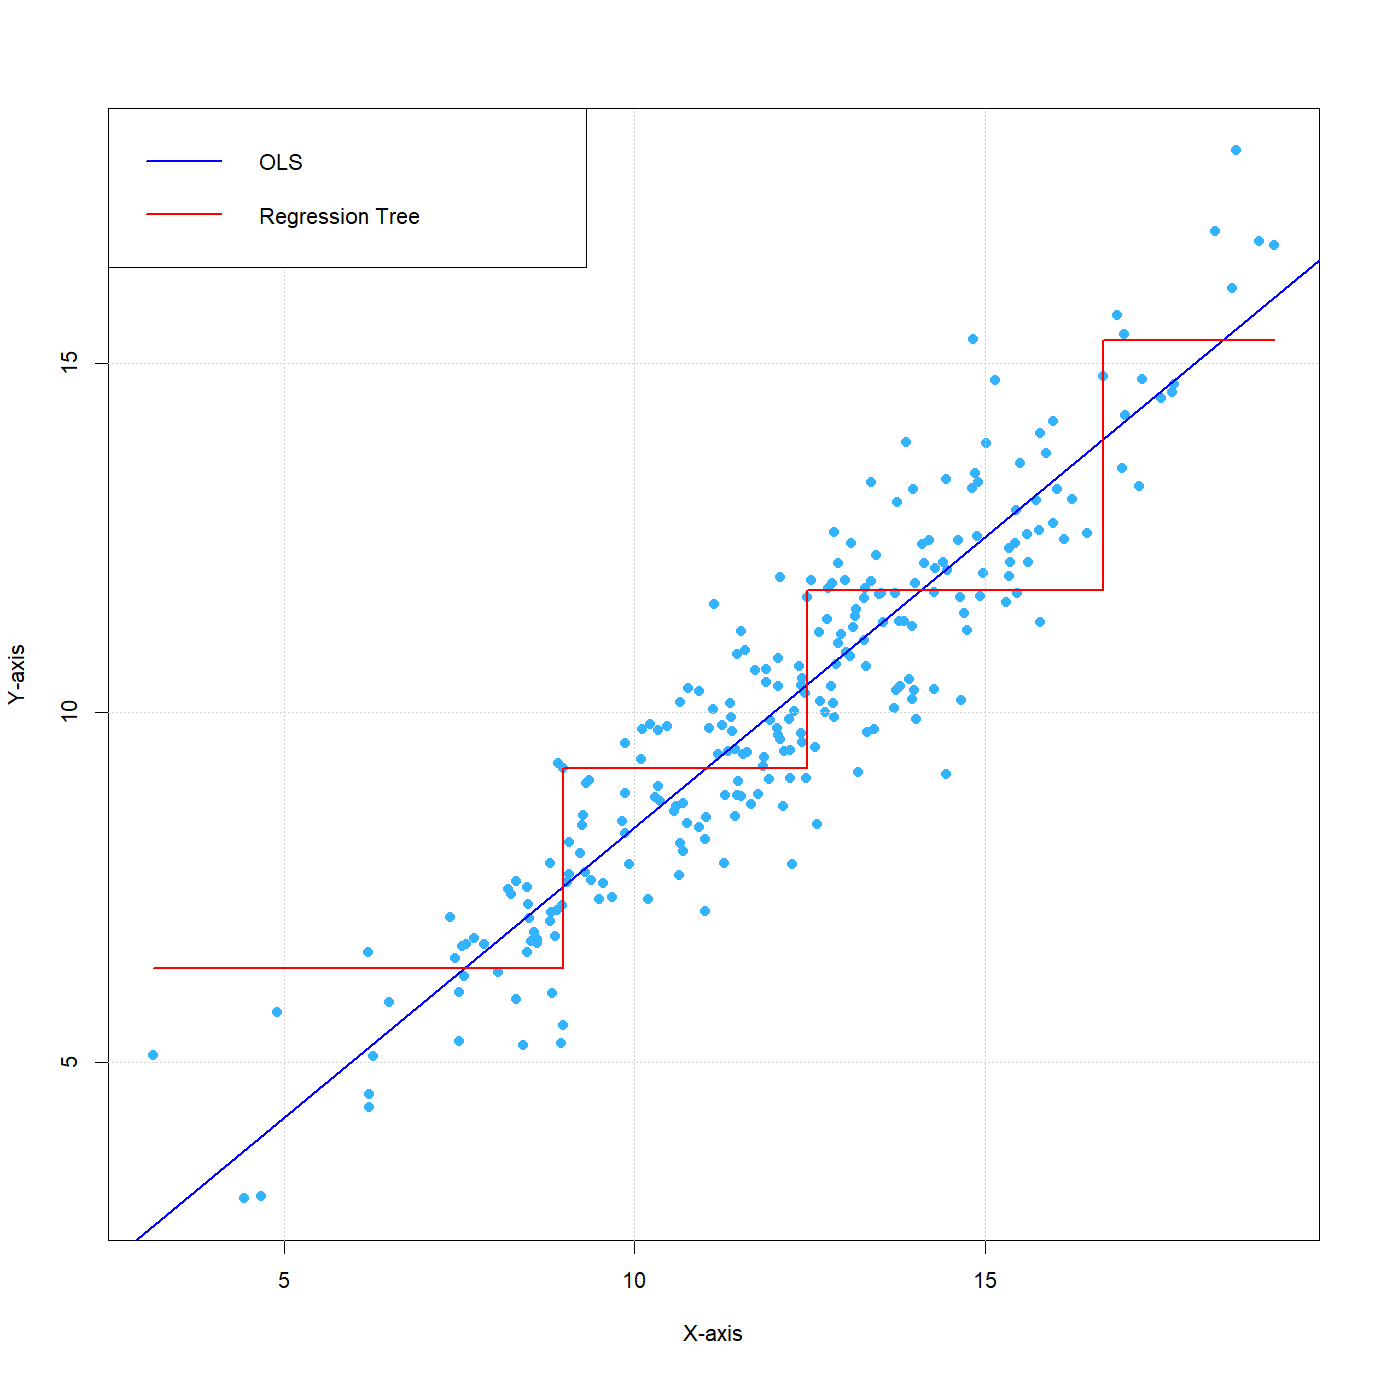
\includegraphics[scale=0.25]{OLS vs Tree.png}
    \caption{Linear Relation between Variables}
\end{figure}


The mean squared error for the Linear regression is: 0.9917
While for the regression tree it is: 1.4935

The linear regression also wins out on intuitiveness. The derivative of the line of best fit can be interpreted as the expected increase in variable y as the x variable increases. While the step function of the regression tree doesn't serve any obvious function. It's just a worse regression.


\subsection{Non-linear Data}
In this second simulation, the data have a non-linear relationship. In this case, I used classification trees instead of regression trees, as this allows using color as our third dimension instead of having to use a three-dimensional plot.

The data was generated using 4 normal distributions with varying variance, in the four corners of the plot. With the North-West and SE being red and the NE and SW distribution producing blue datapoints.

\begin{figure}
    \centering
    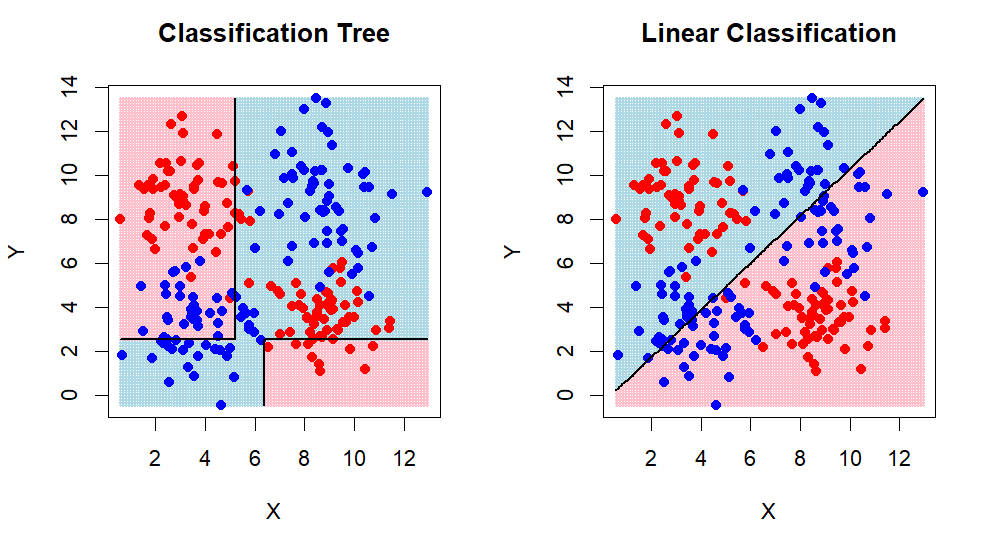
\includegraphics[scale=0.30]{NLD Pred.png}
    \caption{Complex, overfitting Tree}
\end{figure}


Again, we ran the simulation 400 times. In this case, the error rate of the Classification Tree is 37.57\%. While the linear classifier has an error rate of 51.03\%. If this weren't a classification but a regression problem, one can imagine the red data having a high Z value, and the blue data having a low Z value, the result would be much the same. One could imagine a linear regression of the form $Z = x^2 - y^2$ forming a sort of saddle point, but this is not what the typical regression will look like, and especially would this interaction not be captured naturally by the linear model. Whereas the regression trees, because of their recursive nature, can naturally capture interaction effects. By first splitting along one axis and then along a different one, this will happen automatically.

This simulation also shows how Trees capture interaction effects naturally; the fact that a large X value is only indicative of the observation being Red if the Y value is small is naturally captured by the tree.

One could try to showcase more differences between the two methods now, especially on a simulation with more dimensions, seeing how an optimally pruned tree compares against multiple linear regression. But it is more interesting to do this on a real dataset, so we will leave the simulations behind us for now.







Results:
\begin{itemize}
    \item MSE for OLS model: 0.9917 
    \item MSE for regression tree model: 1.4935 
\end{itemize}






\begin{itemize}
    \item Classification Tree MSE: 0.3757
    \item Linear Classification MSE: 0.5103
\end{itemize}





\section{Predicting grades}


Next, I will apply Tree-based methods and also linear regression to a dataset to showcase differences in a more realistic situation. This dataset of student performance includes 649 students and looks at 33 variables.


One can easily train a large tree on the dataset and find the variable importance, to then be better at further analyses. For example, if one does not remove the variables representing previous test scores, practically all the model does is predict final test score based on previous test score, and all other variables are practically irrelevant.


\subsection{Pruning}

The most important thing to do is to use cross-validation and prune your regression tree; otherwise, nothing of interest will be learned as one will have just overfitted on the dataset.

For this, I split the data into training (70\%) and validation (30\%) sets.

It can be useful to prune some trees manually by hand to get an intuitive feeling for how Regression Trees overfit. Instead of using the sophisticated built-in option to automatically perform 10-fold cross-validation and select the best performing tree, I did it by hand first.

Growing a large tree with the complexity parameter (which only allows splits if they cross a certain threshold in error reduction) cp = 0.01, we get a large tree with a Training MSE of 4.521407 and a Validation MSE of 9.026646. So clearly, this tree is overfitting to a significant degree.

\begin{figure}
    \centering
    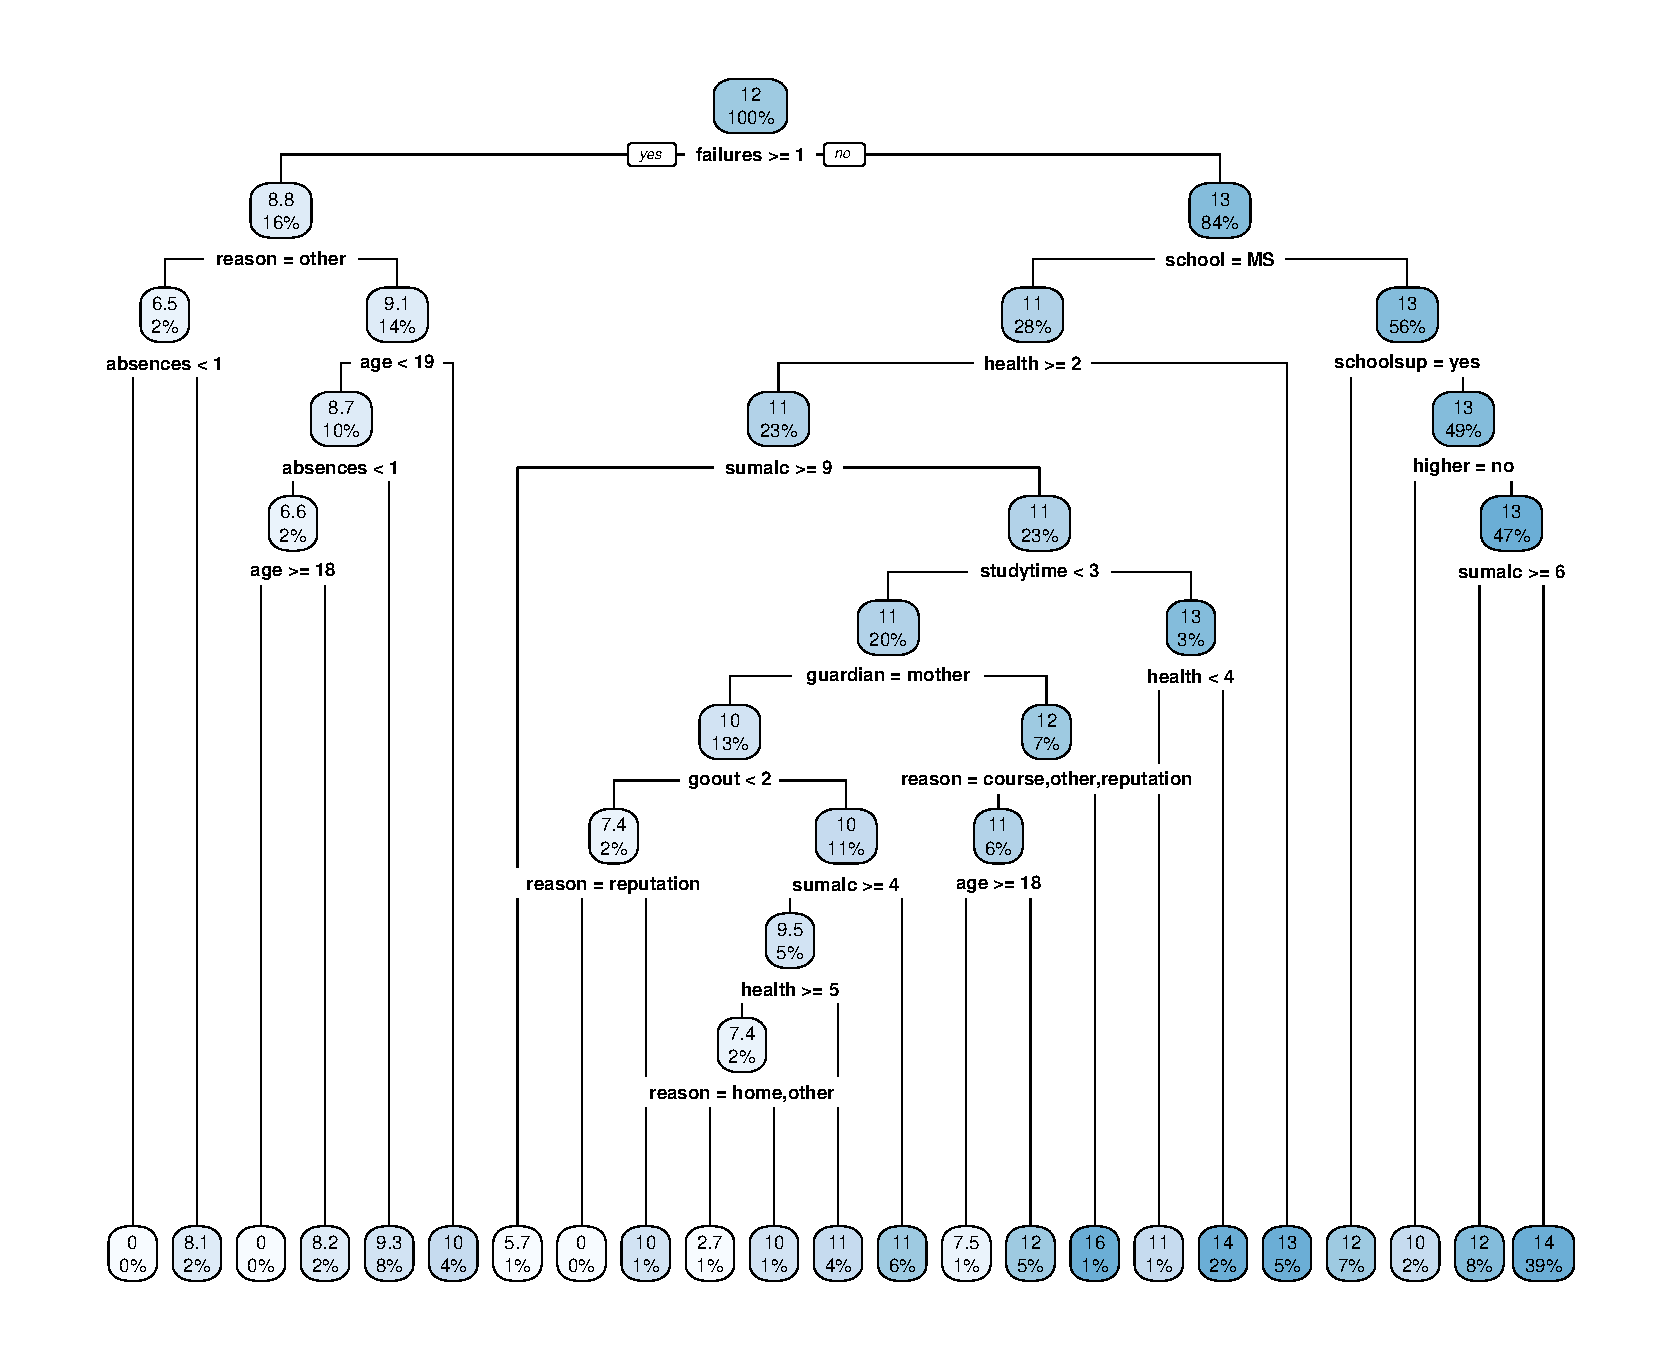
\includegraphics[scale=0.30]{big_manual_tree.pdf}
    \caption{Complex, large Tree}
\end{figure}


Growing a small tree with cp = 0.025 and minsplit = 5 will result in a tree with a Training MSE of 7.840784 and a slightly higher Validation MSE of 8.651296.


\begin{figure}
    \centering
    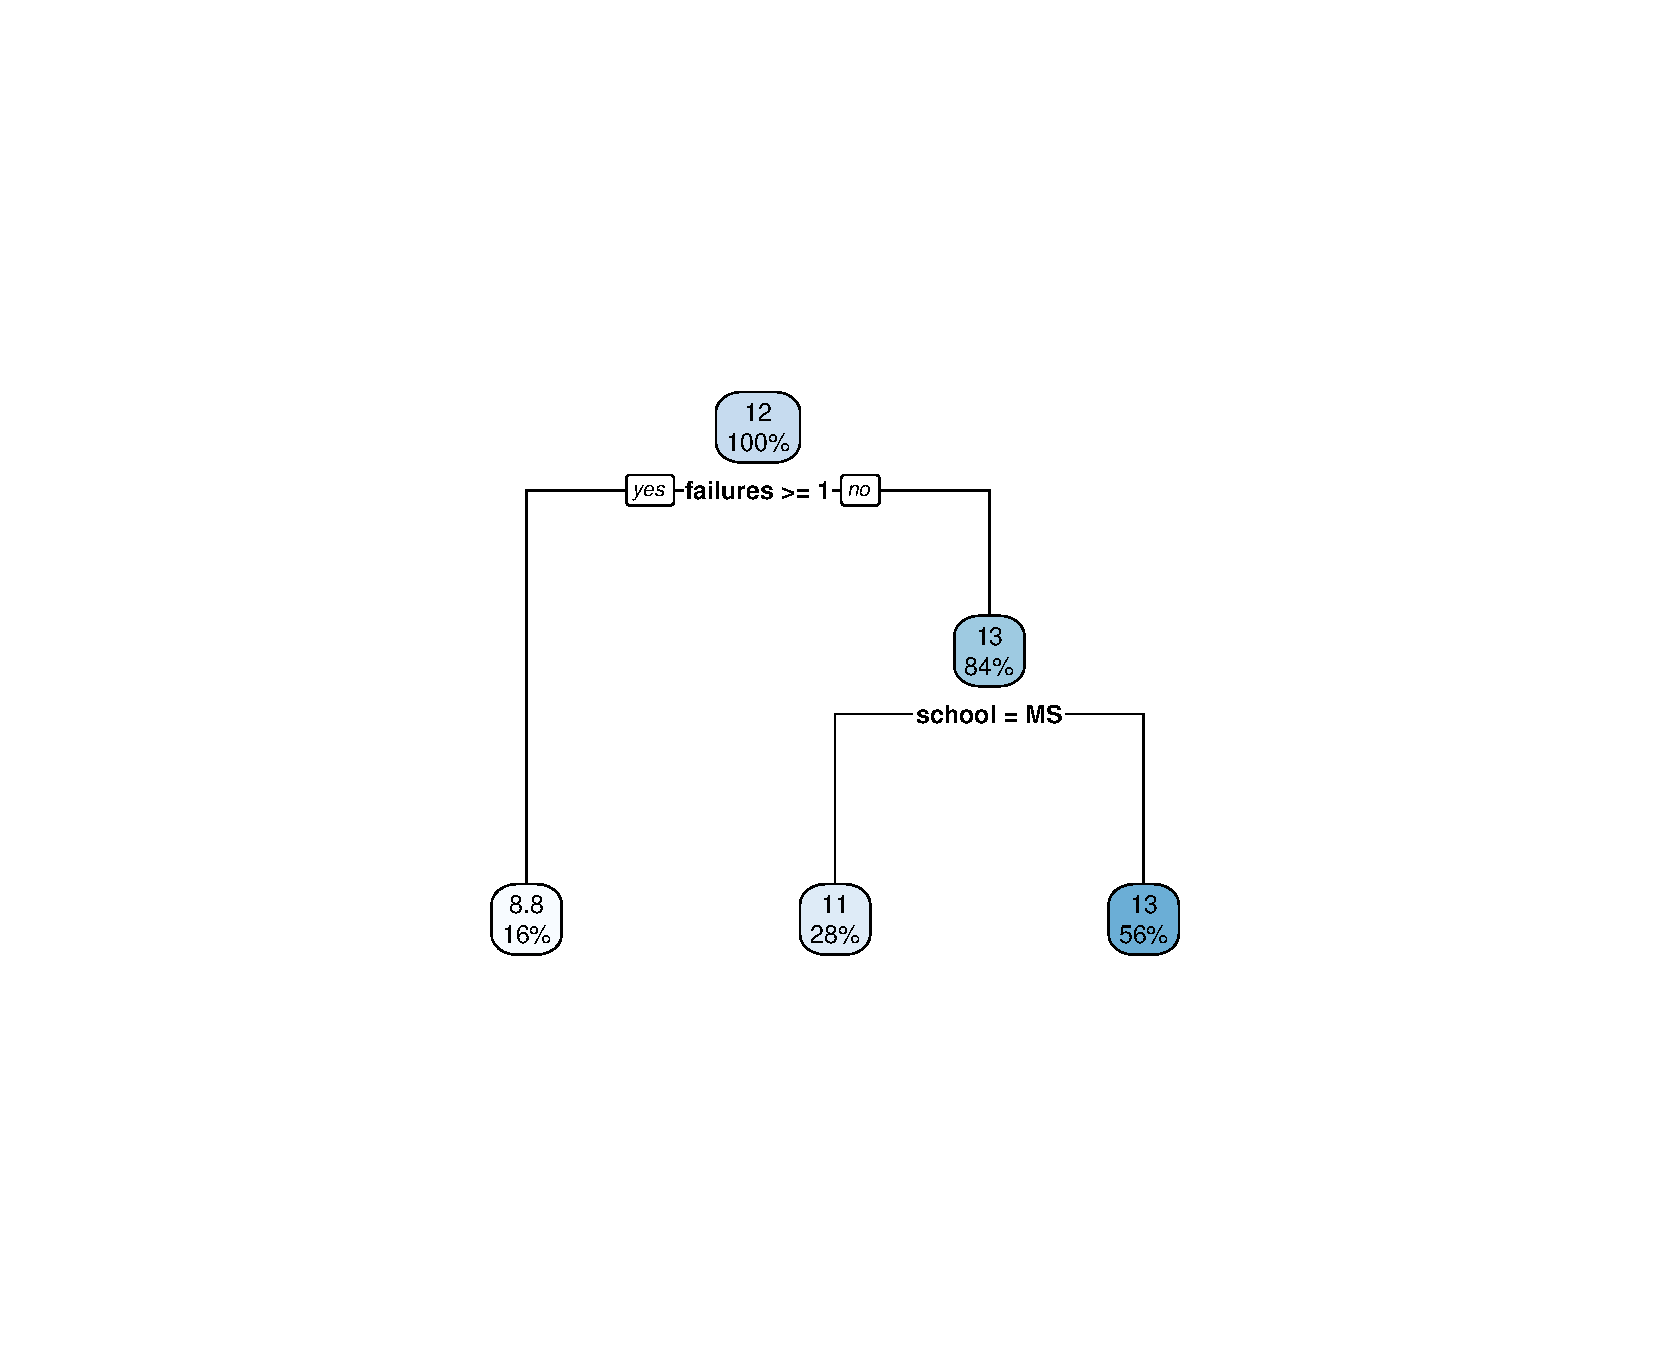
\includegraphics[scale=0.30]{small_manual_tree.pdf}
    \caption{Smaller, better Tree}
\end{figure}



It's somewhat disappointing that this super simple tree outperforms the larger one, but the larger tree is just fitting to the noise of the data, not the real signal.

To find the best possible tree, one should, of course, employ real pruning, automatically evaluated by the machine. This time, I first grew a massive tree that would totally overfit on the training data.

One difficulty here is that even if one is using two datasets to combat overfitting, trying to find the optimal `cp` value that will minimize the error on the test set may result in a situation where, by chance, one of the many different stages of pruning happens to produce a very good result.



This plot nicely shows how pruning can find the optimal Tree, that doesn't overfit too much but still captures some of the datas information.

In the  plot one can nicely see how it could happen by chance that one tree is especially good for some number and if one then chooses that as the tree one is going to work with one overfitting still.
To combat this, I first trained the complex tree on the training set and found the optimal value for `cp` using cross-validation, also on the training set. Only then did I evaluate its performance on the test set.

Sometimes it's so extreme that the optimal pruned tree using cross-validation, once it's evaluated on the test set, gets a MSE on the training data of 5.27211417154088, but on the Test set MSE of 11.4923047228304, clearly overfitting and just lucky during cross-validation.

Here one can see very well how the Cross validation error clearly helps against overfitting, it doesn't decrease monotonically, but still overfits to a large extent. The optimal tree using cross validation has 9 splits while the optimal one on the test error only has 1.


\begin{figure}
    \centering
    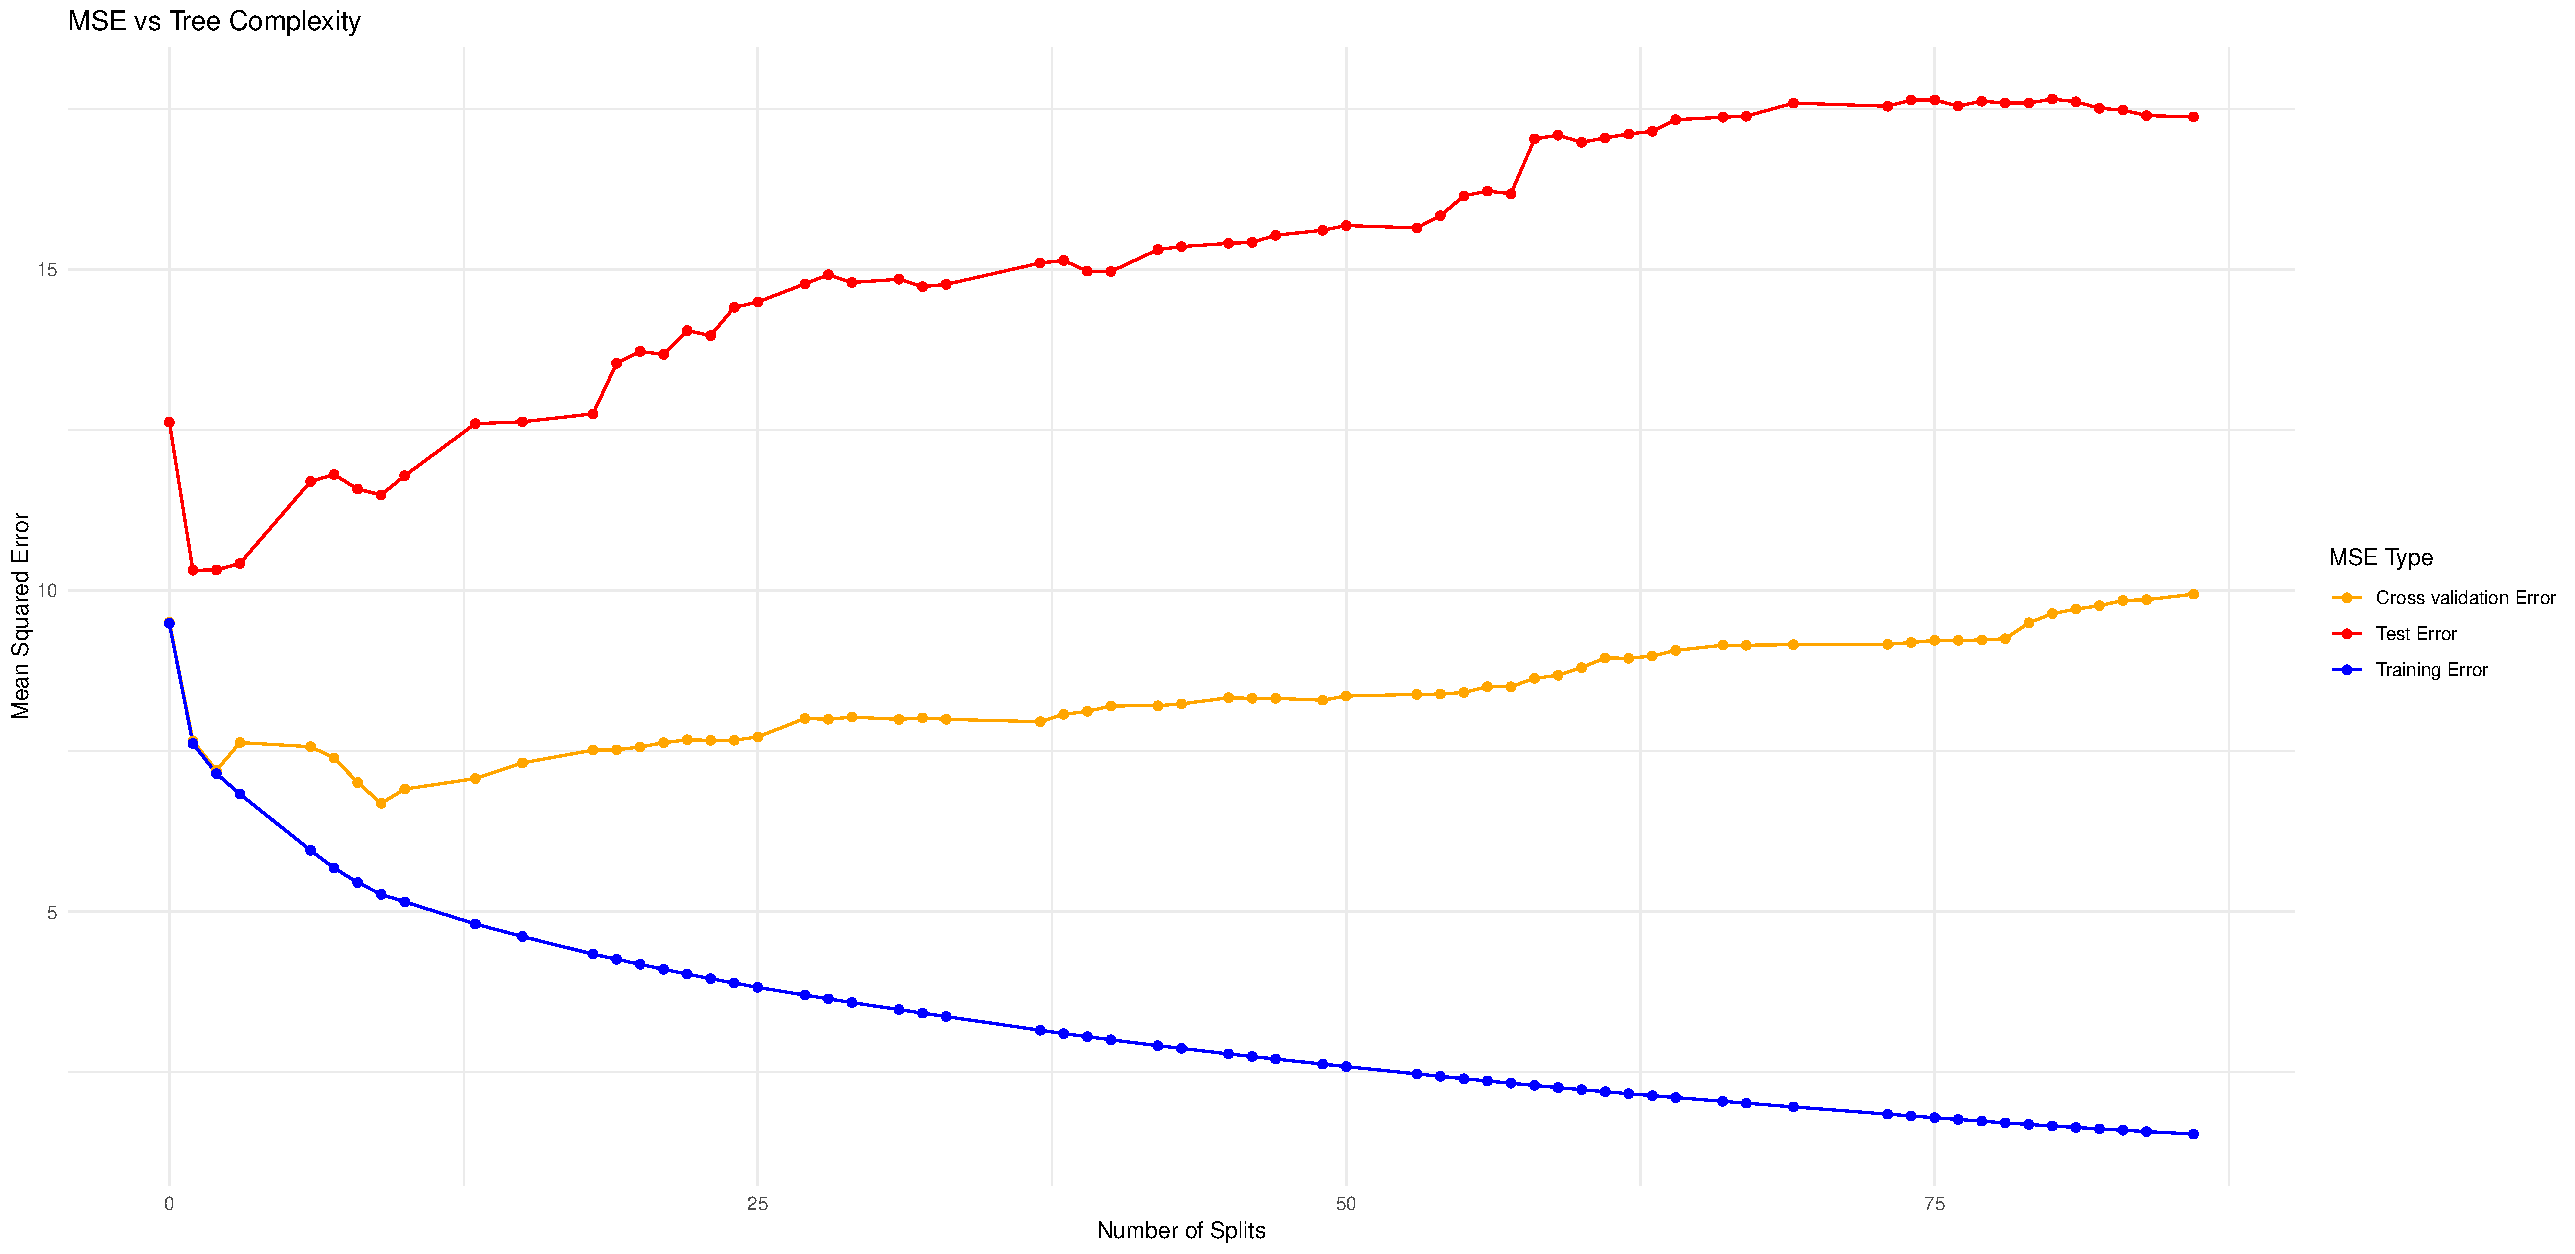
\includegraphics[scale=0.30]{triple_pruning_plot.pdf}
    \caption{Pruning finds the lowest Test error}
\end{figure}

A different problem is that the results can vary quite widley. Different splits in training and test data might lead to MSEs on the test set for the pruned tree between 6.9 and 9. 

And and optimal value for `cp` which in this case is 0.028 and 0.035.


The most typical results will look something like this:

"Complex Tree - Training MSE: 1.71463455830232"
"Complex Tree -     Test MSE: 10.813428171376"
"Pruned Tree  - Training MSE: 8.52684386213971"
"Pruned Tree  -     Test MSE: 8.18867861784212"

The pruned tree performs just one single split on failures, splitting the 15\% of students who have previously failed the exam into one region (Estimate = 8.4) and the 85\% of students with 0 failures into a second region (13 = estimate). This seems like something a human could have also done by hand.

The fact that the test error is lower than the training error should not be surprising; with only 1 split, the tree couldn't overfit even if it tried. It will always make almost the exact same split anyway. It's just chance if it will get a lower or higher error on the test set.



\subsection{Comparing Linear Regression, Regression Trees, and BART}

After examining the tree's performance, it's informative to compare it to the results obtained from linear regression.

Using a 70\%-30\% split and a tree that isn't overfitting, these are the typical results one gets for Regression Trees and multivariate linear regression. Here, the linear regression isn't optimized at all; it's the very first result one gets, without any pruning or attempts to combat overfitting.

Even without any pruning, linear regression outperforms the tree by a wide margin:

\begin{verbatim}
Training MSE   Tree: 8.526844 
Validation MSE Tree: 8.188679 

Training MSE   Regr: 6.787159 
Validation MSE Regr: 6.865478
\end{verbatim}

Invoking Condorcet to assist us, we can use ensemble methods.

Using BART with the default hyperparameters, that is, a burn-in and sampling period of 2000 iterations each and 200 Trees per iteration, results in the following MSEs for BART:

\begin{verbatim}
Training MSE   BART: 5.777039 
Validation MSE BART: 6.52317
\end{verbatim}

Depending on how the data is split into training and test sets, and other random factors, the numbers for all three models can vary quite widely. However, the single Tree is almost always outperformed by linear regression, and BART outperforms them both.

In return, BART is far less easy to interpret than the other two methods. We made no attempt at improving the performance of the regression model. Presumably, its performance can be increased in some way. But there are, of course, also other datasets where complicated ensemble methods significantly outperform linear methods.

\section{Conclusion}

Regression trees are powerful tools for handling non-linear and interactive effects, often outperforming linear regression in these scenarios. They are also very easy to interpret. However, trees require pruning to combat overfitting. Ensemble methods, by averaging independent trees or fitting trees on the residuals, can significantly improve results. BART, in particular, is a sophisticated method offering good results in many scenarios. While regression trees have their strengths, it's important to choose the right tool for each specific data analysis task. Clearly, there is a reason that there are ``about 188,000 results'' on Google Scholar when one searches for ``Regression Tree'' versus ``about 4,320,000 results'' when searching for ``Linear Regression''. Although, especially random forests are quite popular.

The most obvious problem with simple regression trees is that they overfit immediately without doing anything useful. It seems unimaginable to be able to do only one split on a dataset this large, with that many variables. If students who drink more alcohol score slightly less in the Training set, a linear regression could incorporate this slight factor, and it might well be that this also applies in the Test set and improves model performance. If it's not a real effect and just noise, this slight coefficient won't increase Test error by a lot. Whereas the Regression Tree, after having made its initial useful split, can't help find the best optimal split, apparently hyperfocusing on some seemingly useful area that mostly turns out to be just noise.

While BART beats linear regression, it gives up on interpretability for the most part, while linear regression is very interpretable, in a similar way to regression trees. Arguably more so.

In conclusion, regression trees definitely have their applications. As the simulations show, on very non-linear data, even a simple tree can outperform linear regression by a wide margin. But on real-life data, linear regression will often perform better and be more interpretable and useful. Perhaps trees really shine only on data that has very strong interaction effects, more than the single dataset I considered. 

Of course, one can always find datasets more suited for trees to work better than my data, and better methods to determine which is the best method to use. 

This is a very important area of research, and clearly, there are still many open questions.

\newpage


\bibliography{sources}

\end{document}